%----------------------------------------------------------------------------------------
%    PACKAGES AND THEMES
%----------------------------------------------------------------------------------------
\documentclass[aspectratio=169,xcolor=dvipsnames]{beamer}
\makeatletter
\def\input@path{{theme/}}
\makeatother
\usetheme{CleanEasy}
\usepackage[utf8]{inputenc}
\usepackage{lmodern}
\usepackage[T1]{fontenc}
% \usepackage[brazil]{babel}
\usepackage{fix-cm}
\usepackage{amsmath}
\usepackage{mathtools}
\usepackage{listings}
\usepackage[dvipsnames]{xcolor}
\usepackage{hyperref}
\usepackage{graphicx} % Allows including images
\usepackage{booktabs} % Allows the use of \toprule, \midrule and \bottomrule in tables
\usepackage{tikz}
\usetikzlibrary{positioning, shapes, arrows, calc, decorations.pathreplacing, arrows.meta, backgrounds, patterns, overlay-beamer-styles}
\usepackage{etoolbox}
\usepackage{animate}

%----------------------------------------------------------------------------------------
%    LAYOUT CONFIGURATION
%----------------------------------------------------------------------------------------



% Configure code listings
\lstset{
  basicstyle=\ttfamily\small,
  keywordstyle=\color{blue},
  commentstyle=\color{green!60!black},
  stringstyle=\color{red},
  showstringspaces=false,
  breaklines=true,
  frame=single,
  rulecolor=\color{black!30},
  backgroundcolor=\color{black!5},
  numbers=left,
  numberstyle=\tiny\color{black!70},
  numbersep=5pt
}

%----------------------------------------------------------------------------------------
%    TITLE PAGE
%----------------------------------------------------------------------------------------


%---------------------------------------------


\title[Analyzing Ensemble and Backoff Lemmatization of Latin Text]{Analyzing Ensemble and Backoff Lemmatization of Latin Text}

\author[Janaki Mohta]{Janaki Mohta}

\institute[ICR]{
  Institute for Computing in Research
  
}


\vspace{-2cm}\date{July 28, 2025}
% Define positions for logos on title page

\begin{comment}
    \titlegraphic{
  \begin{tikzpicture}[remember picture, overlay]
    % 
    \node[anchor=south west, xshift=0.5cm, yshift=0cm] at (current page.south west) {
      
\includegraphics[height=1.3cm]{logos/CleanEasy-logo1.png}
    };

    % 
    \node[anchor=south west, xshift=2.5cm, yshift=0cm] at (current page.south west) {
      
\includegraphics[height=0.9cm]{logos/CleanEasy-logo2.png}
    };
    
    % 
    \node[anchor=north east, xshift=-0.8cm, yshift=-0.3cm] at (current page.north east) {
      
\includegraphics[height=1.1cm]{logos/CleanEasy-logo3.png}
    };
    
    %
    \node[anchor=north east, xshift=-2.8cm, yshift=-0.3cm] at (current page.north east) {
      
\includegraphics[height=1.4cm]{logos/CleanEasy-logo4.png}
    };
  \end{tikzpicture}
}
\end{comment}


%----------------------------------------------------------------------------------------


\begin{document}

\begin{frame}[plain]
  \titlepage
\end{frame}

\begin{frame}{Background: Linguistics}

    Scientific Study of Language\\
   
\ \\
    Rules for analyzing language --- Computing \\
    Natural Language Processing  (NLP)\\
    
\end{frame}

\begin{frame}[t]{Background: Linguistics}
    \ \\
    Important first step: Normalization\\

    \ \\
    \ \\

    
    \begin{columns}
        \begin{column}{0.5\textwidth}
        \centering
        \large
            Stemming \\ \ \\
           Walking \\
           Walk | ing \\
           \textcolor{ForestGreen}{Walk}
            \\ \ \\
            Thing \\
            Th | ing \\
            \textcolor{red}{Th}

        \end{column}
        \pause
        \begin{column}{0.5\textwidth}
        \centering
            Lemmatization \\
            \ \\
            \centering
            "conventionally defined ‘base’ form" (Sprugnoli et al., 2020) \\ \ \\
             \begin{columns}
            \begin{column}{0.5\textwidth}
            \ \\
            \centering
            \large
            Walking \\
            "Walk" -ing \\
           \textcolor{ForestGreen}{Walk} \\ \ \\
            \end{column}
            
            \begin{column}{0.5\textwidth}
            \centering
            \large
            Thing \\
            "Thing" \\
           \textcolor{ForestGreen}{Thing}
            \end{column}
        \end{columns}
        \end{column}
    \end{columns} 

\end{frame}

\begin{frame}{Linguistics in Latin}

    \begin{columns}
        \begin{column}[t]{0.5\textwidth}
            {\large Strengths}
        \begin{itemize}
            \item Standardization
            \item Precise word forms
        \end{itemize}
        \end{column}
         \begin{column}[t]{0.5\textwidth}
            {\large Weaknesses}
        \begin{itemize}
            \item Many endings
            \item Repeated endings \\
             \ \ \ \ \ \ templum; stem \textcolor{ForestGreen}{templ-} \\
             \ \ \ \ \ \ interdum; stem \textcolor{red}{interd-}
        \end{itemize}
        \end{column}
    \end{columns}

    \ \\ \ \\ \ \\ \ \\
        
    \centering
    {\large Lemmatization stronger choice}
    
\end{frame}

\begin{frame}[t]{CLTK Latin Lemmatization}

 {\large The Lemmatizers}\\
    \begin{itemize}
        \item Dict - Dictionary
        \item Unigram - Training %visualization
        \item Regexp - "Stemmer"
        \item Old Dict - Larger Dictionary
        \item Identity - Failsafe \\%explanation
        \ \ \ \ \ \ templi \rightarrow{} \text{\textcolor{red}{templi}} \\
        \ \ \ \ \ \ \ \ \ \ \ \ interdum \rightarrow{} \text{{\textcolor{ForestGreen}{interdum}}}  \\ \ \\
    \end{itemize}
        {\large Backoff Lemmatization Pipeline}\\
    \ \\
    
\includegraphics[width=1\textwidth] {cltk_backoff_model_v1.png} %include example with a word
    
\end{frame}

\begin{frame}[t]{CLTK Latin Lemmatization}
\ \\

 {\Large Ensemble: Promising Second Option?}\\ \ \\
 Ensemble lemmatization with the Classical Language Toolkit (Burns, 2020) \\ \ \\
    \begin{columns}
        \begin{column}{0.5\textwidth}
                Strong lemmatizers strengthening each other \\
    \ \\
        \end{column}
         \begin{column}{0.5\textwidth}
         \centering
                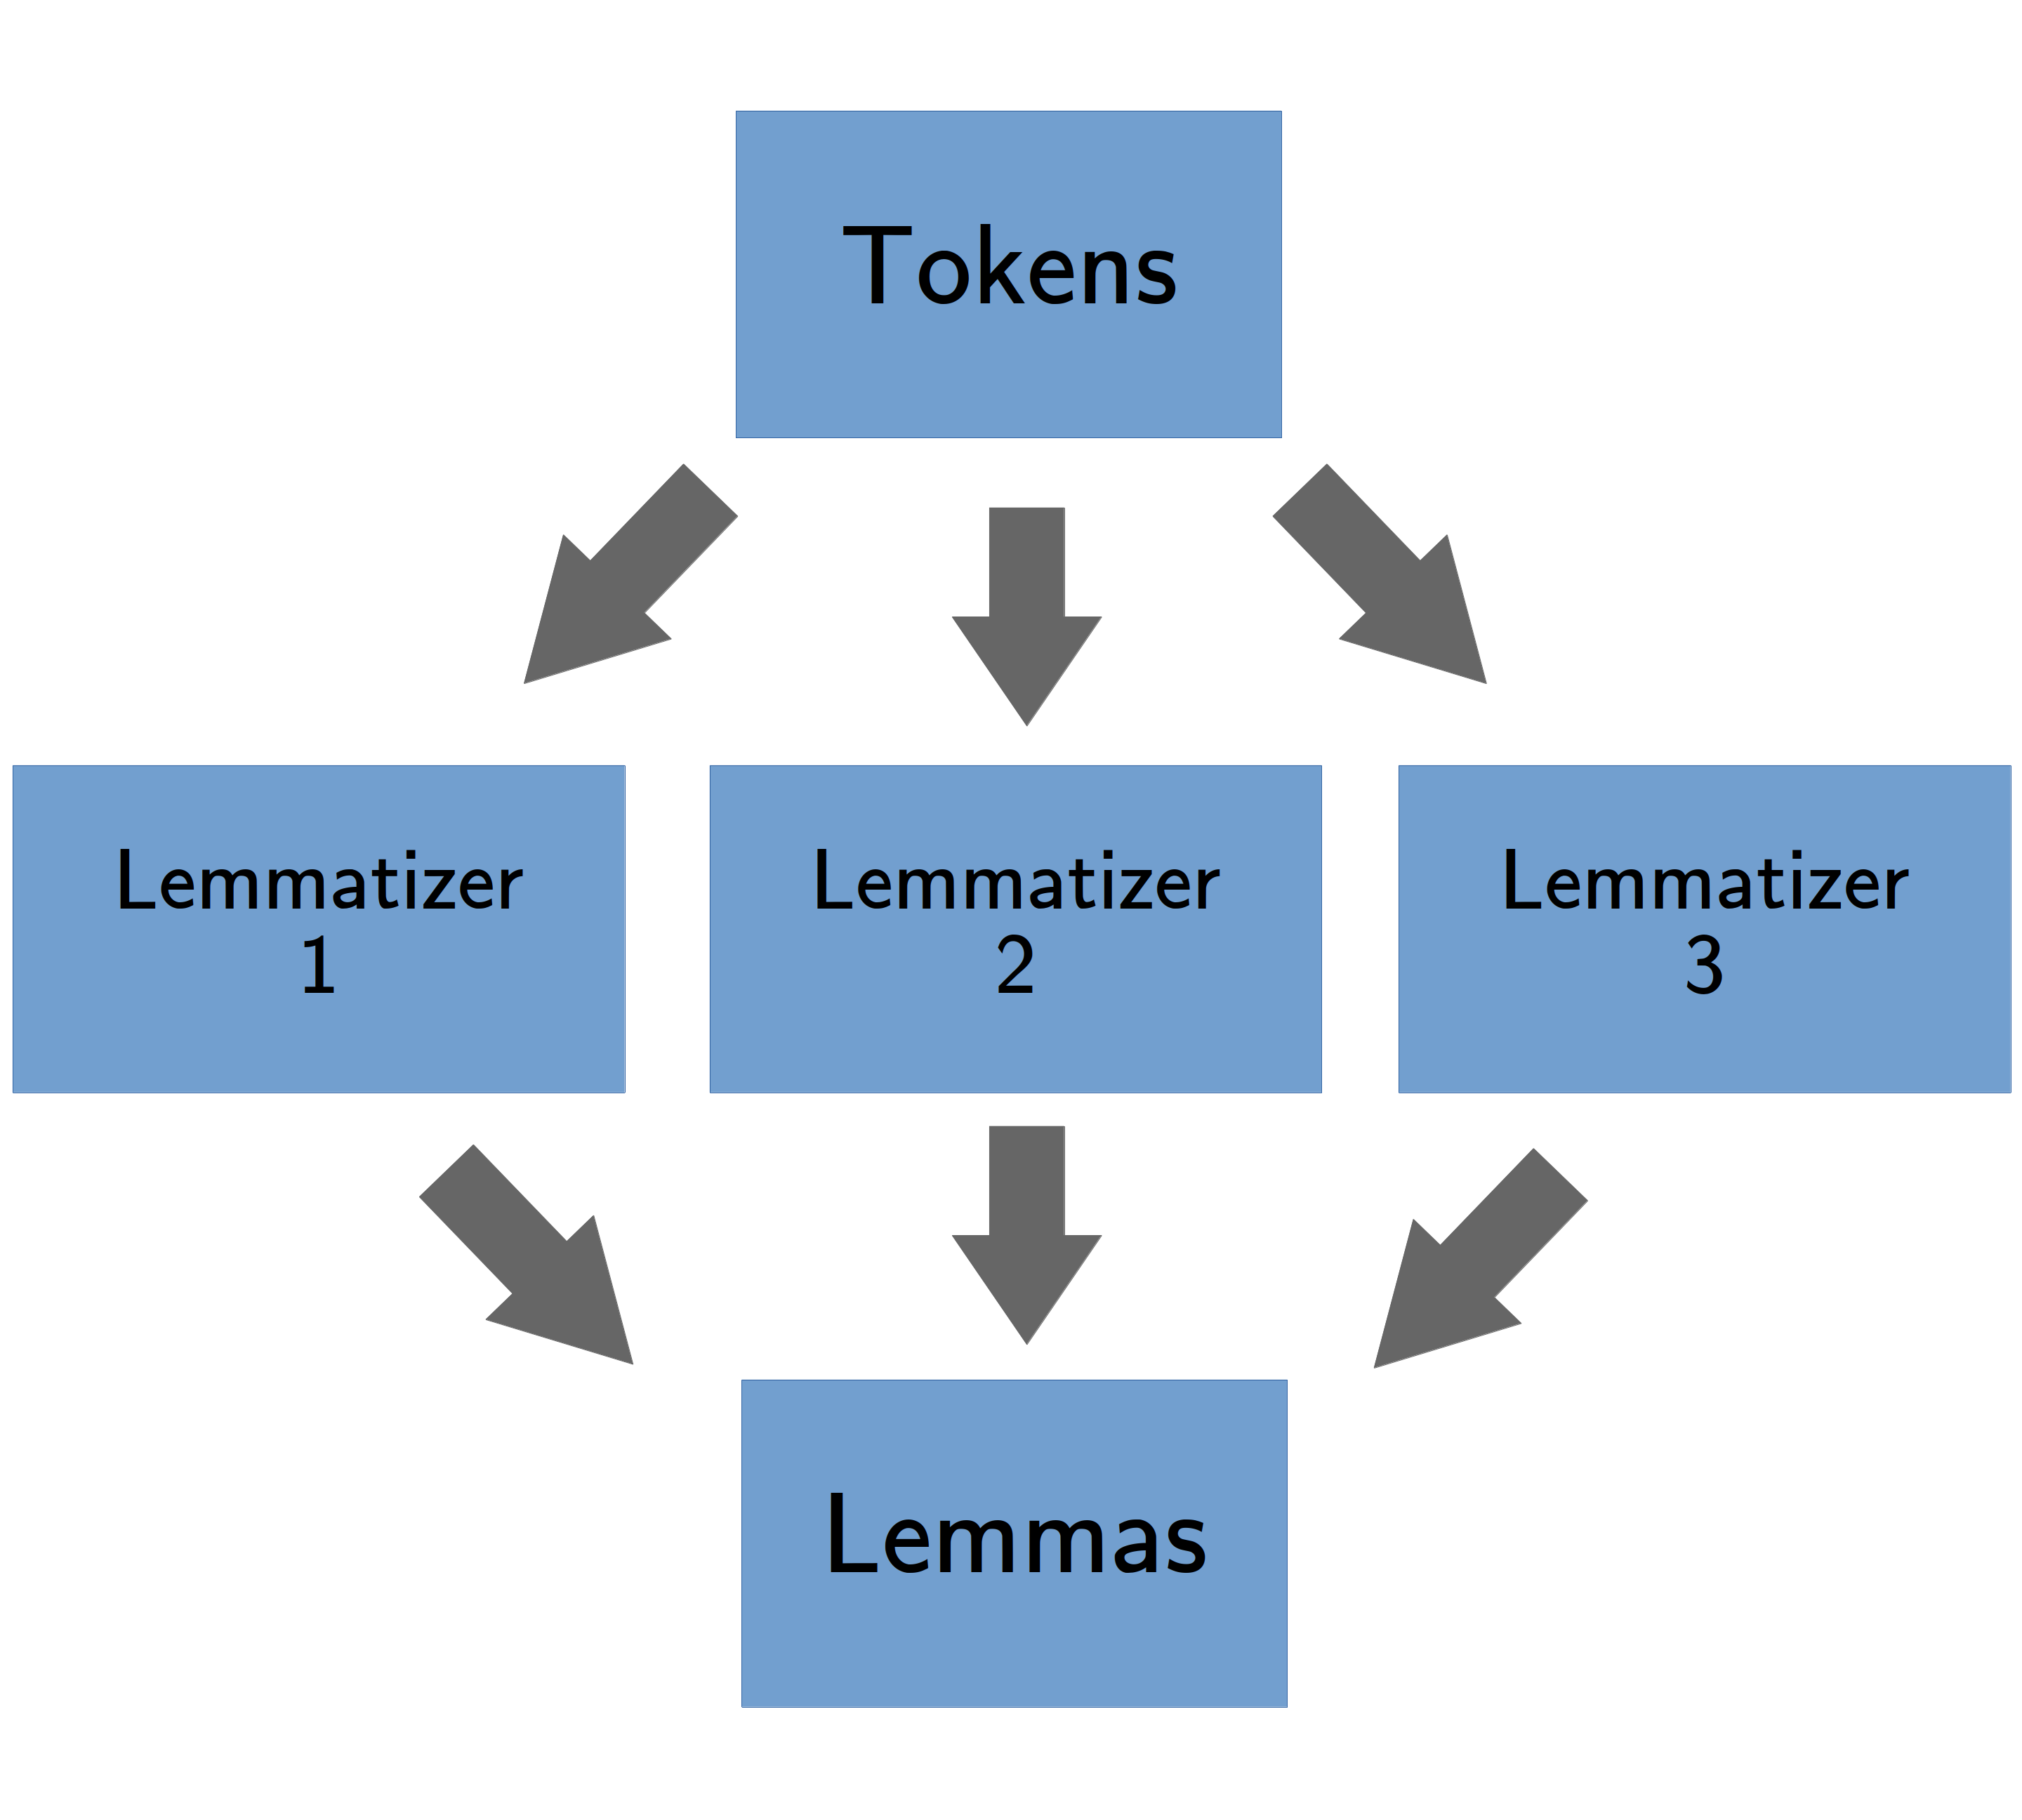
\includegraphics[width=0.7\textwidth]{ensemble_model_v3.png} \\ \ \\
        \end{column}
    \end{columns}
    
\end{frame}

\begin{frame}[t]{CLTK Ensemble Lemmatization}
    Description in paper vs implementation in library \\ \ \\ \ \\ \ \\
    \begin{columns}
        \begin{column}{0.5\textwidth}
            {\large Lemmatizers Offered}\\
            \begin{itemize}
                \item Dict
                \item Unigram
                \item Regexp
                \item Old Dict
            \end{itemize}
        \end{column}
        \begin{column}{0.5\textwidth}
                {\large Potential Benefits}\\
                \begin{itemize}
                    \item Nuance
                    \item Customization
                    \item Expandability
                \end{itemize}
        \end{column}
    \end{columns} 
\ \\ \ \\ \ \\ \ \\ \ \\
{\Large Why hasn't Ensemble overtaken Backoff?}
\end{frame}

\begin{frame}[t]{Preparing for Tests}
\ \\
    Isolating sub-lemmatizers \\ \ \\

    Getting a dataset
    \begin{itemize}
        \item Virgil's \textit{Aeneid}
        \item Cicero's Catilinarian Orations
        \item \textbf{Caesar's \textit{Commentarii de Bello Gallico}}
    \end{itemize}
 \ \\ \ \\
    Manual lemmatization: Time constraints
\end{frame}

\begin{frame}[t]{Testing Dataset Size}
\ \\
    \begin{columns}
        \begin{column}{0.75\textwidth}
           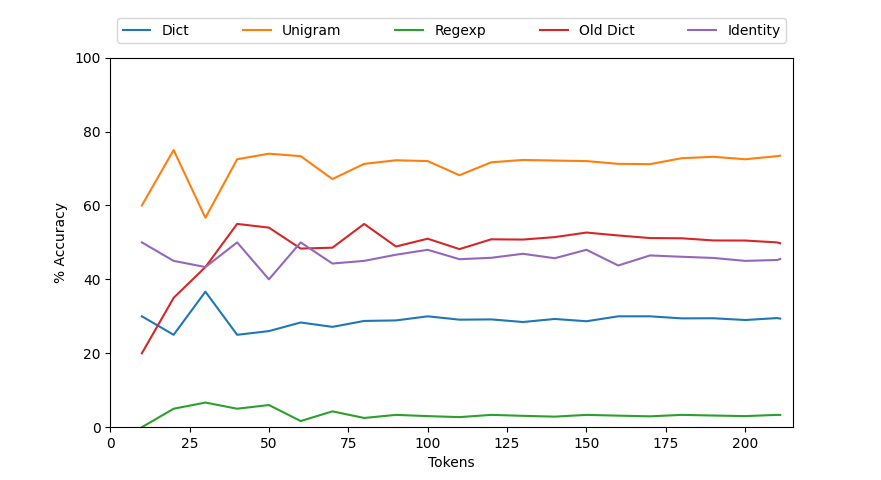
\includegraphics[width=1\textwidth]{accuracy_over_time_v3.png}
        \end{column}
        \begin{column}{0.35\textwidth}
                Random slicing \\ \ \\
                Stabilization: sign of consistency \\ \ \\
                Caveat: Repeated tokens
        \end{column}
    \end{columns} 

\end{frame}

%a little squished both physically and (it seems like) ideas-ly
\begin{frame}[t]{Individual Sub-Lemmatizers}
    \begin{columns}
        \begin{column}{0.6\textwidth}
           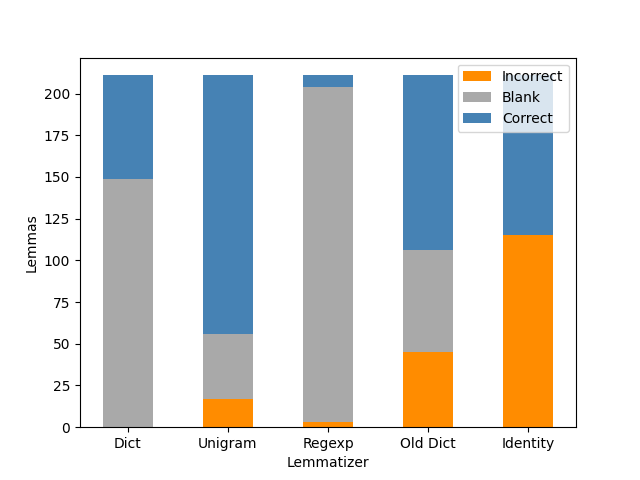
\includegraphics[width=0.9\textwidth]{sub_lemmatizer_performance.png}
        \end{column}
        
        \begin{column}{0.3\textwidth}
        \\ \ \\ \ \\
            \centering
            
\includegraphics[width=0.7\textwidth]{accuracy_ratios_v5.png} \ \\
            \footnotesize
            Correct - Incorrect Ratio (Accuracy Ratio) \\
        \end{column}
    \end{columns} \ \\
    {\Large Why hasn't Ensemble overtaken Backoff?}\\
    Can the Backoff order itself be optimized?
\end{frame}

\begin{frame}[t]{Custom Backoff Pipelines}
\ \\
 \begin{columns}
        \begin{column}{0.5\textwidth}
    
\includegraphics[width=1\textwidth]{custom_pipeline_performances_v3.png}
        \end{column}
        \begin{column}{0.4\textwidth}
            No pipelines as accurate, many pipelines close \\ \ \\
            Worse configuration of the same components
        \end{column}
    \end{columns} 
    \ \\
    {\large Can the Backoff order itself be optimized?} \\
    \ \ \ \ \ \ \ \ General conclusion: No \\
    \ \ \ \ \ \ \ \ Sub-lemmatizers optimized for order

    
\end{frame}

\begin{frame}{Custom Ensemble Pipelines}
\ \\
 \begin{columns}
        \begin{column}{0.55\textwidth}
    
\includegraphics[width=1\textwidth]{ensemble_performances_v2.png}
        \end{column}
        \begin{column}{0.4\textwidth}
            Similar to Backoff: Consistently slightly worse \\ \ \\
            Optimization for task \\ \ \\
            Dict underuse \\ \ \\
            Unigram: "est" \rightarrow{} \text{"sum": 0.993, "edo": 0.007}
        \end{column}
    \end{columns} 

    
\end{frame}

\begin{frame}[t]{A Common Theme}

    \Large{Why hasn't Ensemble overtaken Backoff?}\\
    \large
    Can the Backoff order itself be optimized? \\ \ \\ \ \\ \ \\
    \normalsize 
    The key: Optimization \\ \ \\
    Backoff pipeline specialized \\ \ \\
    Ensemble in this form: Doomed to fail? \\
    \ \ \ \ \ \ \ \  Specialization\\
    \ \ \ \ \ \ \ \      Number of lemmatizers \\

    \ \ \ \ \ \ \ \      Complex weighting --- worse Backoff
\end{frame}

\begin{frame}[t]{Stronger Ensemble Applications}

    \begin{columns}
        \begin{column}{0.5\textwidth}
            Multiple lemmatization pipelines \\ \ \\
            Burns's original proposal
        \end{column}
        \begin{column}{0.5\textwidth}
              \centering
            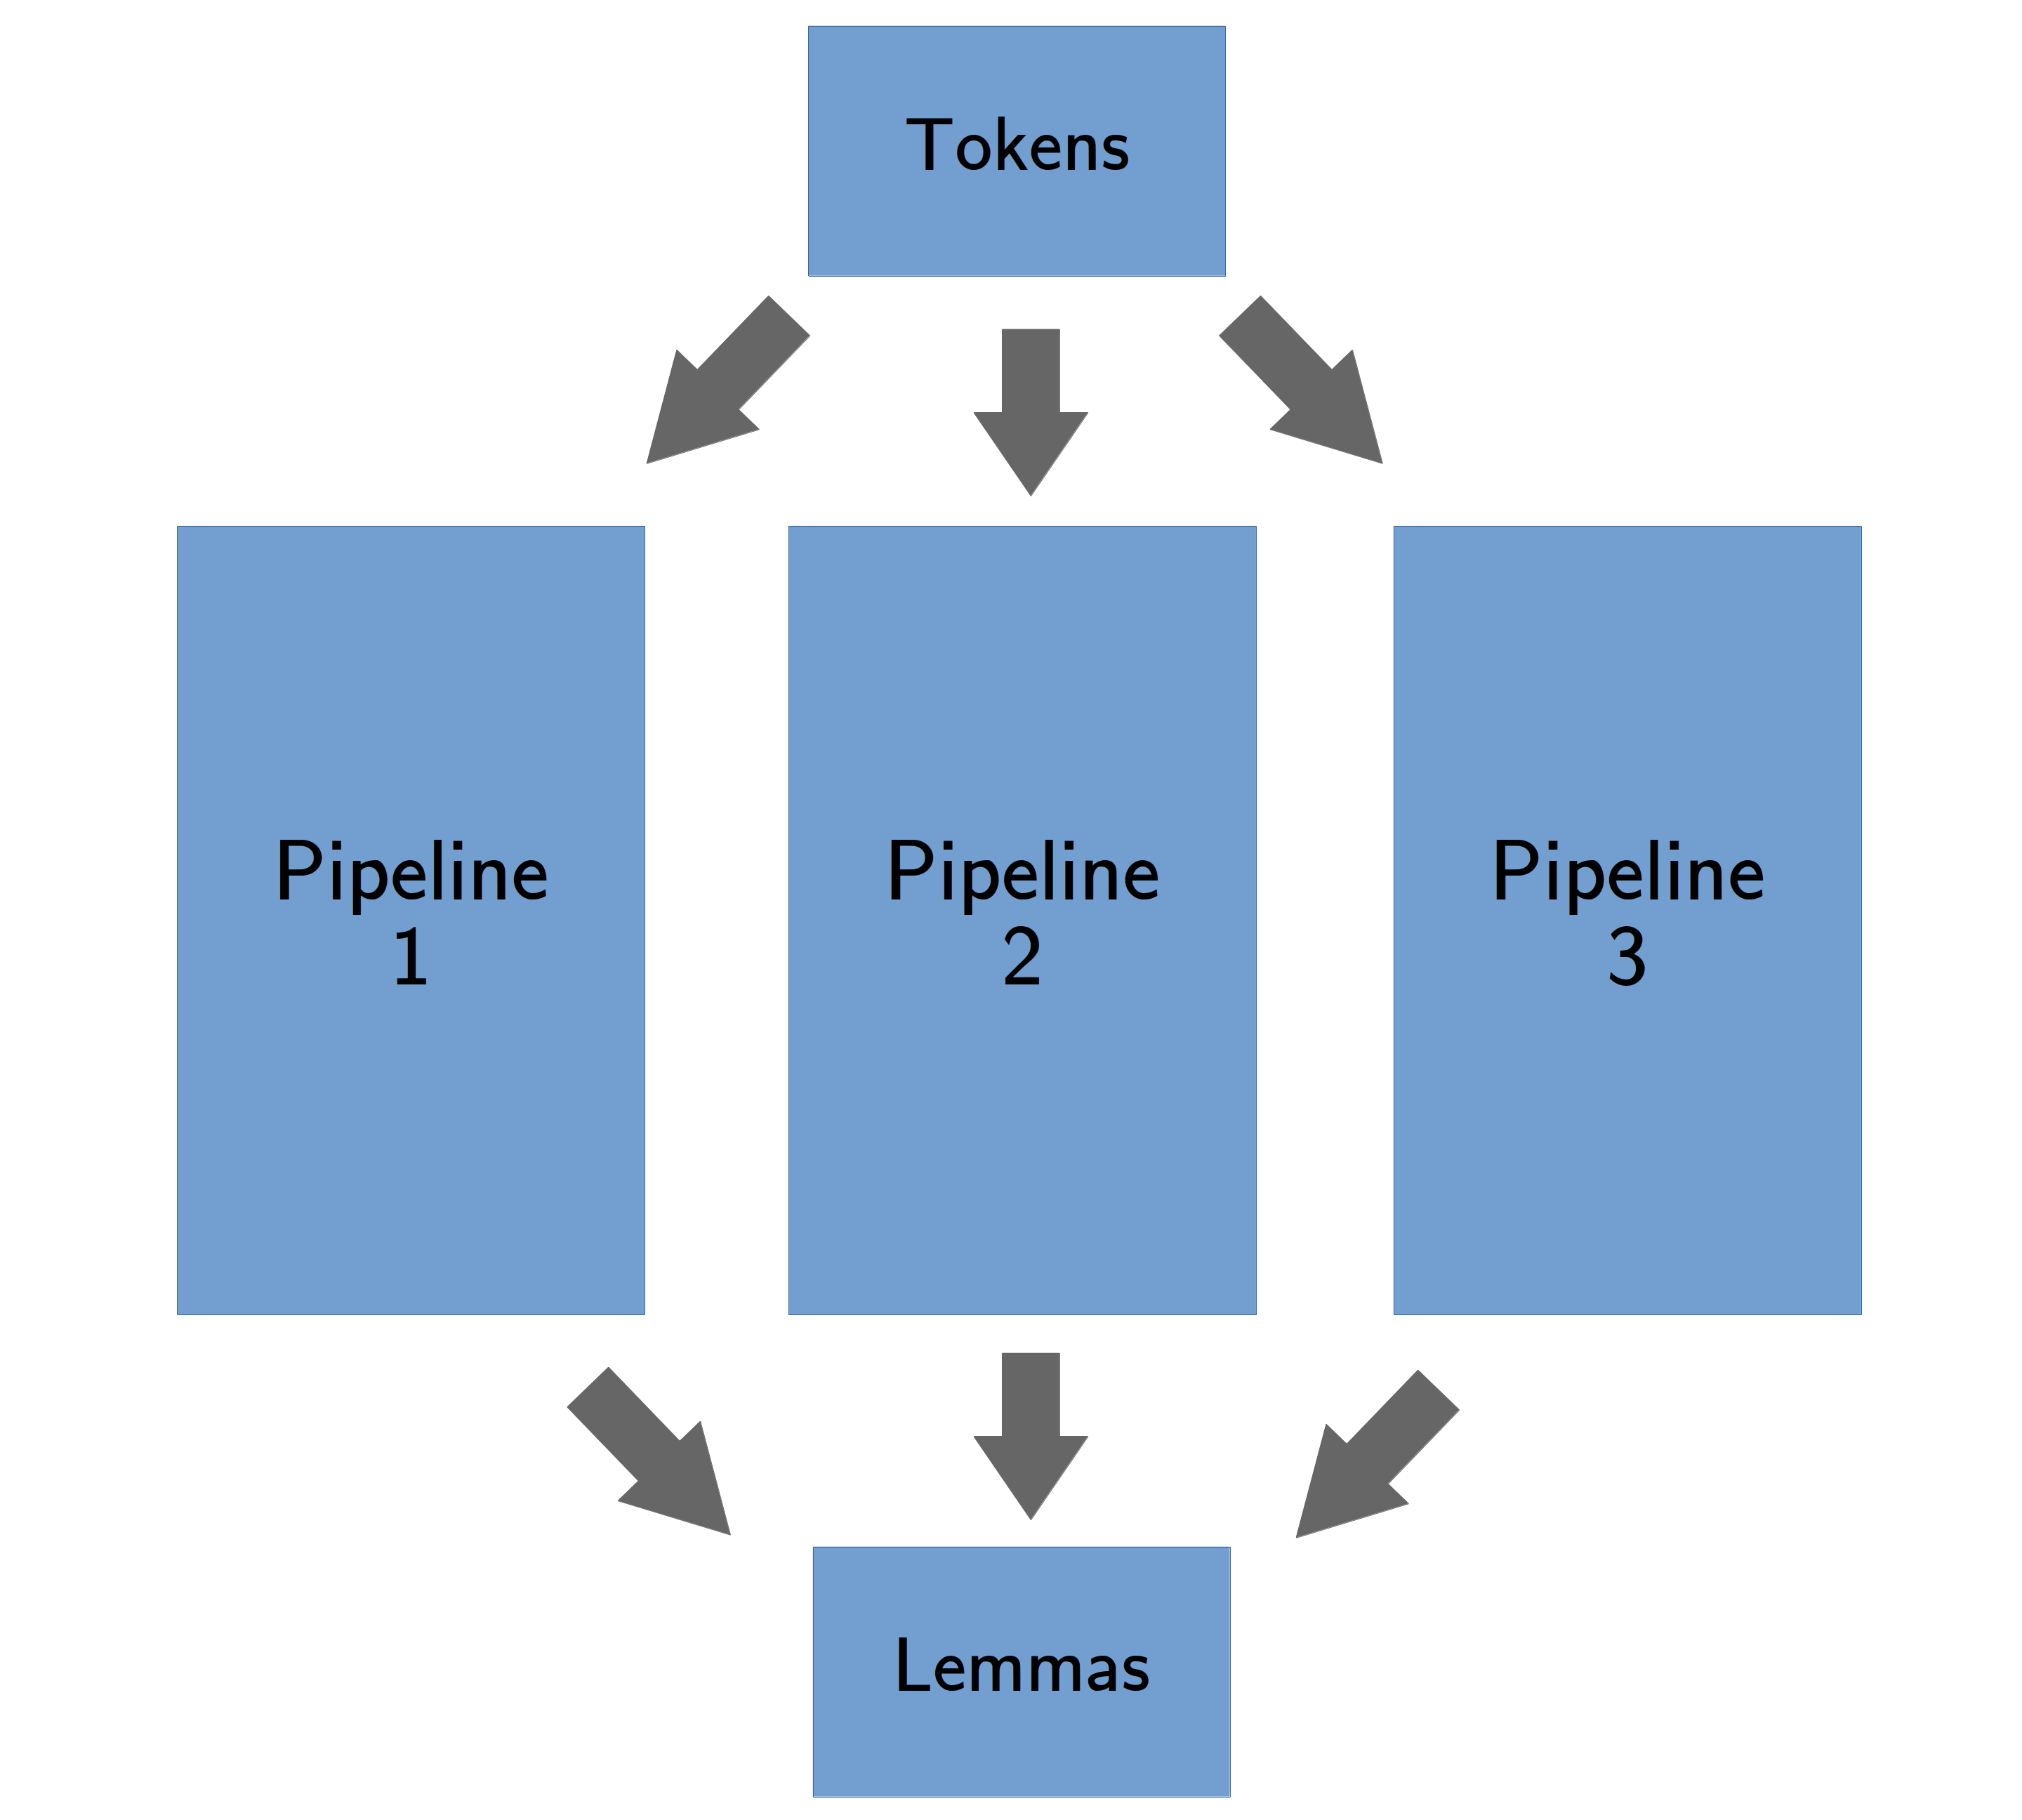
\includegraphics[width=1\textwidth]{ensemble_of_backoffs_model_v4.png} \\ \ \\ \ \\ \ \\ \ \\
        \end{column}
    \end{columns}
           
    
\end{frame}

\begin{frame}[t]{Stronger Ensemble Applications}
             Strengthening segment of Backoff chain\\
                        Strong choice: Unigram \\ \ \\ \ \\ \ \\
            \centering
            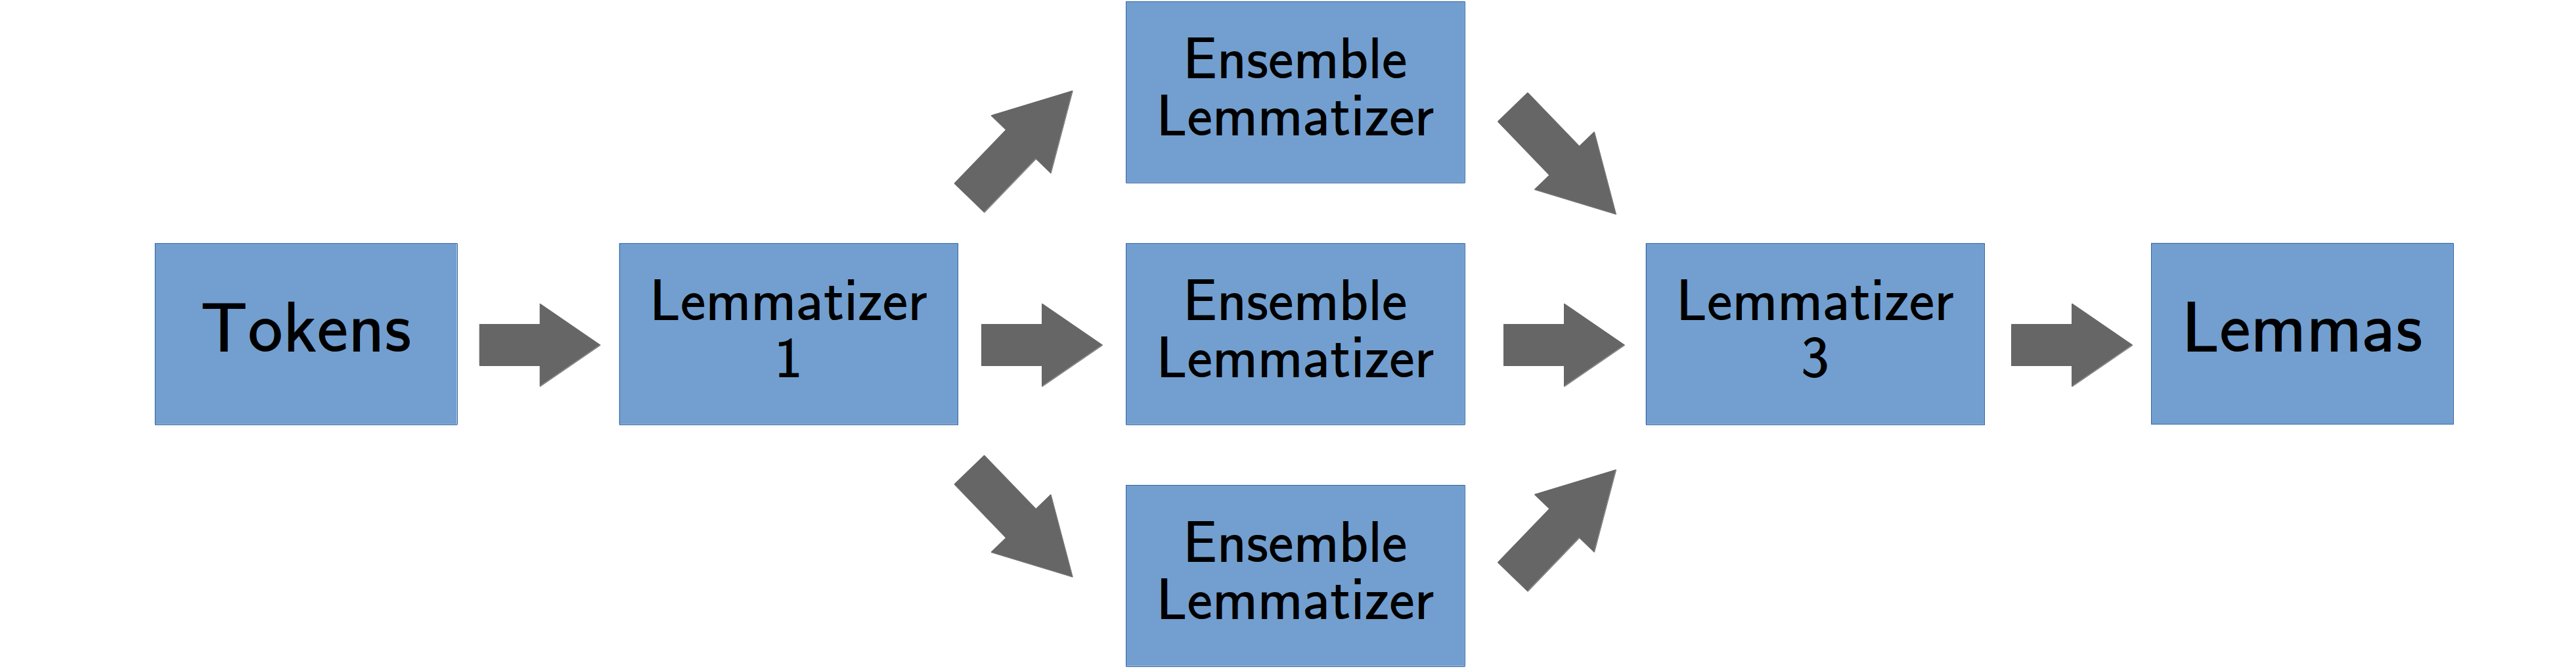
\includegraphics[width=1\textwidth]{backoff_of_ensembles_model_v3.png} \\ \ \\

\end{frame}

\begin{frame}[t]{Next Steps}

\begin{columns}
    \begin{column}{0.5\textwidth}
        Testing Ensemble in stronger forms \\ \ \\
    Application: strengthening complex lemmatizers \\
    \ \ \ \ \ \ \ \ Stronger lemmatizers developed \\
    \ \ \ \ \ \ \ \ Easy increase in performance? \\
    \ \ \ \ \ \ \ \ Potentially diminishing returns
    \end{column}
    \begin{column}{0.5\textwidth}
    \centering
        
\includegraphics[width=1\textwidth]{stanza.png} \\
        
\includegraphics[width=0.7\textwidth]{latincy.png} \\ \ \\
    \end{column}
\end{columns}
    
    
\end{frame}

\begin{frame}{\ }
  \centering \Huge{\textbf{\fontfamily{\rmdefault}\selectfont
  Thank You}}
\end{frame}

\end{document}